% ****** Start of file apssamp.tex ******
%
%   This file is part of the APS files in the REVTeX 4.1 distribution.
%   Version 4.1r of REVTeX, August 2010
%
%   Copyright (c) 2009, 2010 The American Physical Society.
%
%   See the REVTeX 4 README file for restrictions and more information.
%
% TeX'ing this file requires that you have AMS-LaTeX 2.0 installed
% as well as the rest of the prerequisites for REVTeX 4.1
%
% See the REVTeX 4 README file
% It also requires running BibTeX. The commands are as follows:
%
%  1)  latex apssamp.tex
%  2)  bibtex apssamp
%  3)  latex apssamp.tex
%  4)  latex apssamp.tex
%
%
\documentclass[%
%  reprint,
 superscriptaddress,
%groupedaddress,
%unsortedaddress,
%runinaddress,
%frontmatterverbose, 
% preprint,
showpacs,preprintnumbers,
%nofootinbib,
%nobibnotes,
%bibnotes,
 amsmath,
 amssymb,
 aps,
 pra,
% prb,
% rmp,
%prstab,
%prstper,
%floatfix,
showkeys,
onecolumn,
% twocolumn,
notitlepage,
11pt,
% linenumbers,
tightenlines      % uncomment for double space
]{revtex4-1}

\usepackage{graphicx}% Include figure files
\usepackage{dcolumn}% Align table columns on decimal point
\usepackage{bm}% bold math
\usepackage{hyperref}% add hypertext capabilities
%\usepackage[mathlines]{lineno}% Enable numbering of text and display math
%\linenumbers\relax % Commence numbering lines

\usepackage[
% showframe,%Uncomment any one of the following lines to test 
% scale=0.7, 
% marginratio={1:1, 2:3}, ignoreall,% default settings
% text={4.8in, 8in},centering,
% text={6in, 8in},
centering,
a4paper,
margin=2.0cm,
% top=1.in,
% bottom=1.in,
% total={5.6in,8.75in}, % top=1.2in, left=0.9in, includefoot,
% height=10in,
a4paper,
% hmargin={3cm,0.8in},
% marginpar=1in,
% inner=1in,
% outer=1in,
% papersize={6.10in,9.25in}
]{geometry}

\usepackage{fontspec}

% \usepackage{cmbright}
% \DeclareFontShape{OT1}{cmss}{m}{it}{<->ssub*cmss/m/sl}{}
% \renewcommand{\rmdefault}{cmss}
% \renewcommand{\sfdefault}{cmss}

\setsansfont[
BoldFont=ArialBold.ttf,
BoldItalicFont=ArialBoldItalic.ttf,
ItalicFont=ArialItalic.ttf
]{Arial.ttf}
\renewcommand*\familydefault{\sfdefault} 
\setmainfont{Arial}


%%%%%%%%%%%%%%%%%%%%%%%%%%%%%%%%%%%%%%%%%%%%
%%%%%%%%%%%%%%%%%%%%%% COLOR %%%%%%%%%%%%%%%
%%%%%%%%%%%%%%%%%%%%%%%%%%%%%%%%%%%%%%%%%%%%
\usepackage{xcolor}
\usepackage{soul}
\definecolor{reddish}{HTML}{FBB4AE}
\definecolor{blueish}{HTML}{B3CDE3}
\definecolor{magentish}{HTML}{FF00AA}
\definecolor{greenish}{HTML}{a1d99b}
\DeclareRobustCommand{\red}[1]{{\sethlcolor{reddish}\hl{#1}}}
\DeclareRobustCommand{\flow}[1]{\noindent{\sethlcolor{greenish}\hl{\textbf{FLOW}  #1}}}

\usepackage{colortbl}% http://ctan.org/pkg/colortbl
\definecolor{GrayAbstract}{gray}{0.97}
\definecolor{Gray2}{gray}{0.85}
\definecolor{Gray}{gray}{0.95}

\DeclareRobustCommand{\blue}[1]{{\sethlcolor{blueish}\hl{#1}}}
\DeclareRobustCommand{\magenta}[1]{{\sethlcolor{magentish}\hl{#1}}}

% \linespread{1.} 
% \linespread{1.6}
        
%%%% modifying APS template a bit:
% times 
% \usepackage{mathptmx}
% arabic number section
\renewcommand\thesection{\arabic{section}}
\renewcommand\thesubsection{\thesection.\arabic{subsection}}
% section left-side and title style
\usepackage{titlesec}
\titleformat*{\section}{\Large\bfseries}
\titleformat*{\subsection}{\bfseries}
% FIG. -> Fig.
\renewcommand{\figurename}{Fig.}
% spacing after and before section headers
\titlespacing*{\section}{0pt}{1ex plus 1ex minus .5ex}{0.5ex}
\titlespacing*{\subsection}{0pt}{1ex plus 1ex minus .5ex}{0.5ex}
\usepackage{natbib}
\setcitestyle{sort&compress, super}
\definecolor{blueish2}{HTML}{0830Bb}
\hypersetup{colorlinks = true,
            linkcolor = blueish2,
            urlcolor  = blueish2,
            citecolor = blueish2,
            anchorcolor = blueish2}
% section left-side and title style


\makeatletter
\renewcommand*{\fnum@figure}{{\normalfont\bfseries \figurename~\thefigure}}
\makeatother

\setlength{\bibsep}{2mm}
\setlength\bibhang{0.1in}
\usepackage{setspace}
\begin{document}

\title{\Large Machine Learning in Chess}

% \author{NO AUTHORS GIVEN}
\author{Isaac Cheng}
\email{isaaccheng9@gmail.com}

\begin{abstract}
\noindent \textbf{Abstract}

% \textnormal{
\noindent 
(100-200 words)

\end{abstract}

\maketitle

\vspace*{\fill}


\begin{center}
I certify that all material in this dissertation which is not my own work has been identified.
\end{center}
\vspace{1em}

Signature: \hrulefill


\newpage
\section{Introduction}
% The use of computers in chess has been a popular topic of study over the past century or so. 
% Computers are able to perform tasks sequentially incredibly quickly, they generally do not make mistakes, and they have a large capacity for storing information quickly in the form of secondary storage devices. In chess, this means they are able to perform move calculations at orders of magnitudes faster than humans, and they can store large amounts of information about chess games.

Over the past decade, chess has become increasingly significant in popular culture. The rise of full-time streamers on platforms like Twitch has made chess a mainstream form of entertainment. Sponsors have invested substantial sums of money into chess, with platforms such as chess.com incentivising streamers to integrate the game into their schedules. The onset of the COVID-19 pandemic further encouraged this, with people exploring digital forms of entertainment due to lockdown mandates from governments across the globe. 'The Queen's Gambit' was released in 2020, serving as the most poignant example of chess in popular culture yet. People started to take a greater interest in the game, and the number of games played daily on online platforms like chess.com and Lichess has skyrocketed. 

The study of chess has great social importance, as chess games involve cognition and human behaviour that we can apply more generally. For example, social learning theory is a crucial aspect of chess strategy -- players building their chess fundamentals learn from the same material and are thus likely to develop homogeneous habits. People have researched the impact of social learning in the game of Go \cite{beheim2014strategic}, but not for chess.

Strategic board games are good candidates for artificial intelligence research due to their fixed environment. Other games like Go have also undergone extensive studies \cite{muller2002computer}. Chess is an apt game for data mining and machine learning -- the games are well-structured, with a defined search space and comprehensive databases of historical chess games. Literature on chess strategy is centuries-old, but the terabyte-scale exploration of games has only caught on recently. Professional players have started to improve their game using analytics tools like Stockfish. In this project, I will apply data mining and machine learning tools to millions of chess games to understand patterns in how people play chess.

\section{Preliminary Research}
\subsection{Growth in the Popularity of Chess}
While there has been continuous growth in the popularity of chess over the last decade, a significant spike occurred with the pandemic and the release of 'The Queen's Gambit'. Some people have researched Lichess databases to demonstrate this, such as in the chessOpeningStats repository (see figure 1) \cite{chessOpeningStats}. However, there is a lack of formal academic research on this topic -- the closest is a thesis that investigates the influence of Beth and their qualitative effects on how viewers in the Netherlands and United States view chess \cite{lowie2021big}, but this does not provide quantifiable results.

\begin{figure}
\caption{Popularity of Lichess in Number of Games Played Daily \cite{chessOpeningStats}}
\begin{center}
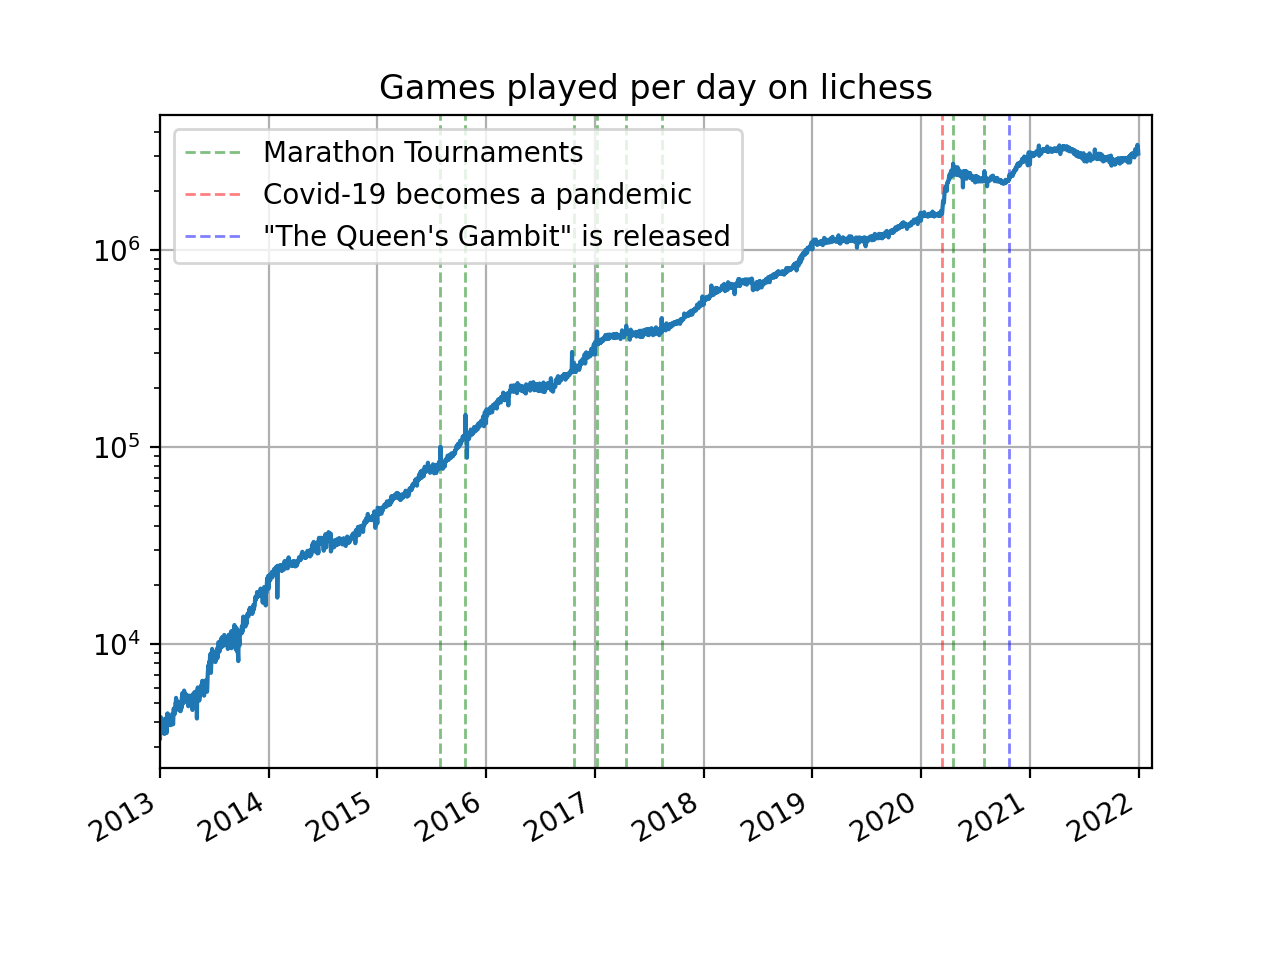
\includegraphics[width=10cm]{images/Lichess Number of Games Played Per Day.png}
\end{center}
\end{figure}

\subsection{History of Computer Chess}
Since the first digital computer was switched on 1945, programmers have sought to build a machine that could defeat the world chess champion \cite{earlyComputerChessHistory}. In 1948, Alan Turing worked with David Champernowne (an economist and mathematician) to create a machine routine for playing chess, dubbed the 'Turochamp' \cite{turingalan}. They did not have a machine, so they simulated the machine's behaviour by hand with a pen and pencil \cite{turingalan}. Champernowne reported that his wife, who was a beginner at chess, took on the machine and lost \cite{copeland2005turing}. A year later in 1949, Claude Shannon wrote a paper that described a computer that could play chess -- his idea was to focus on analysing the seven most likely moves from the current position, and branching from each of these positions into the next seven most likely replies from the opposition, and so forth until the computer runs out of memory \cite{shannon1950xxii}. The first chess program was eventually implemented in November 1951 by Dietrich Prinz. However, unlike Turing's Turochamp, Prinz's program could not complete a full game of chess and used exhaustive search to play moves rather than a heuristic \cite{copeland2005turing}.

The first computer to beat a world champion was IBM's Deep Blue, which defeated Garry Kasparov over a six-game match in 1997 \cite{seirawan1997implications}. Deep Blue was a supercomputer that was able to perform 200 million calculations per second \cite{strogatz2018one}. It was the first computer to use a heuristic search algorithm, which is a method of searching for a solution to a problem by evaluating possible solutions and choosing the best one. By this point, chess engines were stronger than human players, yet they still lacked a deep understanding of the game. Deep Blue's victory was accredited to its brute-force ability -- its over-reliance on this was demonstrated in the first game of their match, as it sacrificed Kasparov's sacrifice of a rook for a bishop, only to lose 16 moves later \cite{strogatz2018one}.

[WRITE EXPLANATION OF STOCKFISH]

Recently, researchers at DeepMind have developed their machine-learning algorithms to master chess alongside other strategic games such as shogi and Go with their AlphaZero machine-learning algorithm \cite{silver2018general}. It was based on their recent AlphaGo Zero program, which achieved superhuman performance using an algorithm based solely on reinforcement learning, with no human data, guidance, or domain knowledge beyond the rules of Go \cite{silver2017mastering}. Likewise, AlphaZero started with no knowledge of chess (nor any of the other strategy games) beyond the basic rules and became the best chess player (human or computer) in the world within hours of learning by playing millions of games \cite{strogatz2018one}. AlphaZero's chess abilities were tested by playing against Stockfish, a chess engine that is considered to be the strongest chess engine in the world. AlphaZero was able to beat Stockfish 8-0 in a match of 8 games \cite{silver2018general}. AlphaZero's victory was attributed to its ability to learn from its mistakes, which is a key aspect of machine learning. It implements a general-purpose Monte-Carlo tree search algorithm, which simulates random games to find the best move \cite{silver2017mastering2}. It also uses a neural network to evaluate the board position, which is a technique that is used in many machine learning algorithms.

[WRITE EXPLANATION OF RECENT SCANDAL REGARDING HANS NIEMANN]

\subsection{Piece Valuation}

\subsection{Social Learning Theory}


\section{Project Specification}
\subsection{Requirements Analysis}
Machine learning in chess covers a broad range of topics, so it is crucial to scope design and development systematically. We will start exploring simple, wide-spanning areas to build a baseline – this may include answering questions such as:

\begin{itemize}
    \item What are the most common chess openings and their success rates?
    \item What are the most popular chess openings over time?
    \item What is the distribution of ELO ratings on a given online platform?
\end{itemize}

Then, we will build up to more complex questions using previous findings. Questions may include:
\begin{itemize}
    \item What are the best counters against particular openings?
    \item To what degree is social learning theory evident in chess?
    \item How good are existing metrics for predicting win probability in chess games?
\end{itemize}

It is also important to outline what will be out of the project's scope. There is a vast range of chess game variants like Chess960 (also known as Fischer random chess), King of the Hill, and Antichess [CITATION NEEDED]. However, they would all introduce significant overhead to our research as they change the fundamental rules and theories of the game. We will not include them in the project to avoid scope creep and maintain a strong focus on the standard variant. In addition, we will not be creating a chess bot that plays games -- we will instead focus on generating insights to understand patterns in chess strategy.

\subsection{Design}
A large data set is paramount to performing machine learning effectively. We will be using Lichess as our data source. They provide an open database of standard-rated games played on lichess.org every month in PGN (Portable Game Notation) format [CITATION NEEDED], which is the standard for recording chess games [CITATION NEEDED]. Lichess is one of the two mainstream platforms for playing chess online (alongside chess.com), which means they provide a large sample to analyse each month -- October 2022 includes over 90 million games.

We will use Python 3.11.0 because Python the de facto standard for data science [CITATION NEEDED] and that is the latest version at the time of writing. The python-chess library has emerged as the most popular for PGN parsing alongside other features -- it has over 1,900 stars on GitHub and is maintained regularly [CITATION NEEDED]. It will accompany the Python Stockfish library, the best and most popular chess engine available to the public [CITATION NEEDED] -- this enables us to integrate the Stockfish engine with Python to analyse positions and generate insights. In addition, we will use industry-standard Python libraries such as seaborn for graph visualisations, pandas for data frames, and NumPy for mathematical analysis.

\subsection{Project Risks}
There are very few risks in the project. The main risk is that the data set is not large enough to provide meaningful insights. However, this is unlikely to be an issue as Lichess provides a large data set every month, and there is already a history of monthly data from January 2013 onwards. The file sizes for Lichess' latest monthly data sets are huge, measuring at 30 GB for the compressed October 2022 download, and 214 GB when uncompressed. The computational analysis for this project will take place on my personal laptop, which is an M1 Max MacBook Pro 16 (2021) with 32 GB of RAM and 1 TB of SSD storage. If the lack of storage space becomes an issue when analysing multiple months' worth of data sets, we could look at using high-speed external solid state drives or using another machine. The latter solution would involve a high-performance desktop computer running a Linux distribution provided by Chico Camargo, which could provide further benefits such as more powerful GPU accelerated computation to streamline our process.

Another risk is that the data set is not representative of the entire chess community. However, this is unlikely to be an issue as Lichess is one of the two mainstream platforms for playing chess online (alongside chess.com), which means they provide a large sample to analyse each month. Lichess is a free platform, which means that it is accessible to a wide range of people. While it would be ideal to also obtain games from chess.com to cover the two main platforms, this is infeasible as they do not provide an open database like Lichess.

\subsection{Ethical and Legal Issues}

\subsection{Development}
Downloading the data is a straightforward process. As aforementioned, we will download monthly games from the Lichess Open Database (provided in compressed form), extract the games from the PGN file, and load them using python-chess. This library will enable us to read the game and navigate to the part we want to analyse. We will start by navigating to the final position of the games. Then, we will get the FEN (Forsyth-Edwards Notation) string, the standard notation for describing a chess game's board position [CITATION NEEDED]. 

Once we have the position, we will analyse it using the Stockfish library. It provides information from the game, including the centipawn score. Stockfish computes the centipawn score using static evaluation of the board position and applying the mini-max algorithm and alpha-beta pruning [CITATION NEEDED]. It measures a white's advantage, where a centipawn equals 1/100 of a pawn [CITATION NEEDED]. Hence, a score of 100 means that white has a pawn's worth of advantage, whereas a score of -100 indicates a pawn's advantage for black. If a player has a significant advantage, Stockfish may find a forced mate -- this means that one player can checkmate the other, regardless of the other player's moves [CITATION NEEDED]. In this case, it will represent the score with either '\#{x}' or '\#{-x}', where x is the number of moves from a checkmate -- the former means white can checkmate black, and the latter means black can checkmate white. Note that this also includes 0 if the game ended due to a checkmate occurring on that move.

Before performing data analysis on the results, we will filter and segment the data according to how the game ended -- this is important because most rated Lichess games are games with a time limit [CITATION NEEDED]. In these games, a player loses the game regardless of their position when they run out of time. It is a common situation that a player loses the game on time despite having an advantageous position on the board [CITATION NEEDED] -- this is an example of the types of games we may want to filter out, as they may add unnecessary noise to the data. On a similar note, games with shorter time limits may have different patterns to others, as time management skills become a more significant factor. We will also differentiate between games that ended from checkmate and games where a player resigned -- the former may be more indicative, as a player resigning is effectively extrapolating the rest of the game and deciding that they will lose.

Next, we will analyse the data to investigate our questions. The simple questions will provide the foundation for our investigations and may not require machine learning, whereas the more complex questions that form the bulk of our project will involve it. For example, identifying the degree to which social learning theory is evident in chess may become a feature importance problem. A reasonable hypothesis is that social learning theory takes place to a greater degree for popular openings, as there is substantially more educational material for them. Thus, we could use feature selection methods such as information gain and variance thresholding to identify the features of games containing less popular openings.

Finally, we will create visualisations of our results to demonstrate them in a manner that is easier to understand. We will plot a bar chart to show the most popular chess openings by percentage and their win rates, as well as a bar chart to demonstrate the distribution of ELO ratings in Lichess. Meanwhile, a line graph will show the most popular chess openings over time. These visualisations for the results of our simple questions will help readers by providing context for further studies on more complex topics. Using the same example as the previous paragraph, we could plot bar charts to compare the importance of different features of games containing less popular openings.

\subsection{Evaluation}

\section{Conclusion}

\bibliographystyle{ieeetr.bst}
\bibliography{main}
\end{document}
